%%%%%%%%%%%%%%%%%%%%%%%%%%%%%%%%%%%%%%%%%
% FRI Data Science_report LaTeX Template
% Version 1.0 (28/1/2020)
% 
% Jure Demšar (jure.demsar@fri.uni-lj.si)
%
% Based on MicromouseSymp article template by:
% Mathias Legrand (legrand.mathias@gmail.com) 
% With extensive modifications by:
% Antonio Valente (antonio.luis.valente@gmail.com)
%
% License:
% CC BY-NC-SA 3.0 (http://creativecommons.org/licenses/by-nc-sa/3.0/)
%
%%%%%%%%%%%%%%%%%%%%%%%%%%%%%%%%%%%%%%%%%


%----------------------------------------------------------------------------------------
%	PACKAGES AND OTHER DOCUMENT CONFIGURATIONS
%----------------------------------------------------------------------------------------
\documentclass[fleqn,moreauthors,10pt]{ds_report}
\usepackage[english]{babel}

% added this
\usepackage{multirow}
\newcommand{\STAB}[1]{\begin{tabular}{@{}c@{}}#1\end{tabular}}

\graphicspath{{fig/}}




%----------------------------------------------------------------------------------------
%	ARTICLE INFORMATION
%----------------------------------------------------------------------------------------

% Header
\JournalInfo{Natural Language Processing 2023}

% Interim or final report
% \Archive{Second submission report} 
\Archive{Final report} 

% Article title
\PaperTitle{Slovenian Language Assistant for Virtual Conversations (SLAVC)} 

% Authors (student competitors) and their info
\Authors{Luka Škodnik, Robert Jutreša, Valter Hudovernik}

% Advisors
\affiliation{\textit{Advisors: doc. dr. Slavko Žitnik}}

% Keywords
\Keywords{Large Language Models, Machine Translation, Conversational AI, Slovene, Question Answering}
\newcommand{\keywordname}{Keywords}


%----------------------------------------------------------------------------------------
%	ABSTRACT
%----------------------------------------------------------------------------------------

\Abstract{
% Slavko je car!
}

%----------------------------------------------------------------------------------------

\begin{document}

% Makes all text pages the same height
\flushbottom 

% Print the title and abstract box
\maketitle 

% Removes page numbering from the first page
\thispagestyle{empty} 

%----------------------------------------------------------------------------------------
%	ARTICLE CONTENTS
%----------------------------------------------------------------------------------------

\section*{Introduction}
	Natural Language Processing (NLP) is an exciting field of Artificial Intelligence that focuses on teaching machines how to understand and respond to human language. 
    In this report, we will discuss our project for the Natural Language Processing course 2022/23, where we aim to develop a Slovenian Conversational Agent called Slovenian Language Assistant for Virtual Conversations  or SLAVC for short.
    % We will provide an overview of our preliminary research, discuss our idea to use a GPT-based model, and explore various data sources that we plan to use to train our model.
    We will provide an overview of our preliminary research, current implementation and explore various data sources that we plan to use and discuss possible models to train or finetune our model.
    % Finally, we will discuss the importance of estimating the amount of data required to train a model effectively.

    
\section*{Related Work}

% Attention & Transformers
\subsection*{Transformers \& Large Language Models}
Attention \cite{vaswani2017attention} is a key component of transformer models, which are widely used in natural language processing tasks such as language translation and text summarization.
It is also a part of many modern large language models (LLM) that we will use during this project.
In transformer models, attention mechanisms allow the model to focus on the most relevant parts of the input sequence at each step of processing.
This is achieved by assigning weights to each element in the input sequence based on its relevance to the current step.
By doing so, the transformer can capture long-range dependencies between different parts of the input sequence, which is particularly important for language processing.

% SloBERTa
SloBERTa \cite{ulvcar2021sloberta} is a Slovene large language model. It is a large pre-trained masked language model based on the BERT architecture. The authors trained the model on a large corpus of Slovene text and evaluated it on various downstream tasks such as text classification, named entity recognition, and part-of-speech tagging. The results show that SloBERTa outperforms existing Slovene language models and achieves competitive performance with state-of-the-art multilingual language models. 

% Instruct GPT
We examine the alignment of language model paradigm using reinforcement learning such as InstructGPT \cite{ouyang2022training}. However due to the lack of resources we instead focus our attention to using already compiled high quality datasets for a one-time training of our model. However their work points out the total number of collective prompts used in training their model, which was $77k$. This gives us an approximate estimate of how much data to use in the fine-tuning process. Additionally they discuss deduplication, however in future works such as \cite{alpaca} have pointed out that repeating prompts is not a big issue.
%% IS THIS TRUE Valter, ARE YOU BULLSHITTING? source: Yannick Kilcher video 

\subsection*{Datasets}
% 3P
The P3 dataset is a collection of prompted English datasets covering a diverse set of NLP tasks. The use of prompts allows for the creation of consistent and standardized data examples across different datasets, which can facilitate the development of new models and the comparison of results across different tasks \cite{bach2022promptsource}. 

% TV Series Subtitles
A corpus of automatically annotated TV series subtitles for dialogue construction was developed in \cite{tv_series_subtitles}. The authors used a combination of rule-based and machine-learning techniques to identify speaker turns and assign speaker identities. They evaluated their method on a corpus of subtitled TV series episodes and achieved high accuracy in speaker identification and turn-taking recognition. The resulting corpus was used for various downstream tasks such as emotion recognition and dialogue act classification.

% GOS
GOS \cite{Verdonik2013} is a reference corpus of spoken Slovene language. The methodology used to collect the corpus involved recording conversations of native Slovene speakers in various domains such as business, education, and social interactions. The transcription process involved annotating the recordings with orthographic, phonetic, and prosodic information. The resulting corpus was used for various research tasks such as acoustic modeling, speaker recognition, and speech synthesis. 

% Alpaca
Alpaca \cite{alpaca} by Standford University is a set consisting of a data generation procedure, dataset, and training recipe. It is a fine tuned model from 7B LLaMA \cite{touvron2023llama} on 52K instruction-following data generated by the techniques in the Self-Instruct \cite{wang2022selfinstruct} paper, with some modifications. In a preliminary human evaluation, it was found that the Alpaca 7B model behaves similarly to the GPT-3 model on the Self-Instruct instruction-following evaluation suite.

% BLOOM
BLOOM \cite{scao2022bloom} a multilingual LLM  was trained on the ROOTS corpus \cite{roots}, amounting to 1.61 terabytes of text that span 46 natural languages and 13 programming languages. Unfortunately Slovenian is not one of the available languages. However, due to vast collections of datasets available such as  Hugging Face datasets \cite{lhoest2021datasets}, we focus on developing tools for robust translation in order to translate the large amounts of available data to Slovenian in order to facilitate the development of a conversational LLM.


% SuperGLUE
SuperGLUE \cite{wang2019superglue} is a benchmark for evaluating the performance of natural language understanding models. It consists of eight challenging natural language understanding tasks, including both textual entailment and commonsense reasoning tasks. The benchmark is designed to test the ability of models to handle more complex linguistic phenomena and to generalize to new examples. The authors compare the performance of several state-of-the-art models on SuperGLUE and find that there is still a significant gap between the best models and human performance.

% UnifiedQA Slo
Logar and Šikonja (2022) \cite{logar2022unified} discuss the challenges of question answering for less-resourced languages and presents an adaptation of the English UnifiedQA approach to the Slovene language. The adaptation uses encoder-decoder transformer models (SloT5 and mT5) to handle different question-answering formats, and existing Slovene adaptations of four datasets, as well as machine translation of the MCTest dataset. The study shows that a general model can perform at least as well as specialized models for answering questions in different formats. However, the performance of the Slovene model still lags behind that of English, and cross-lingual transfer from English is used to improve the results.

% OpenAssistant
The paper "OpenAssistant: Aligning Large Language Models with Human Preferences using Open-Source Conversations" \cite{köpf2023openassistant} presents a new corpus of human-generated, human-annotated assistant-style conversations called OpenAssistant Conversations. The corpus consists of 161,443 messages distributed across 66,497 conversation trees, in 35 different languages, annotated with 461,292 quality ratings, and was created through a worldwide crowd-sourcing effort involving over 13,500 volunteers. The authors also release their code and data under fully permissive licenses, making their work easily accessible to the wider research community. We choose to adapt this dataset for training of a Slovene conversational Assistant. The structure of the dataset is depicted in Figure~\ref{fig:dataset}, on which we comment further in the following section.

\begin{figure}[ht]\centering
	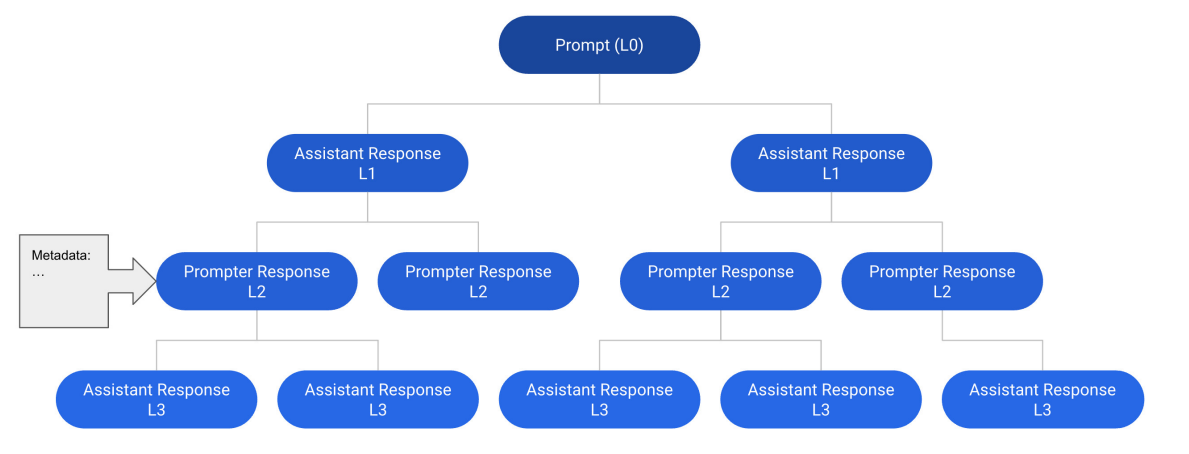
\includegraphics[width=\linewidth]{fig/dataset.png}
	\caption{\textbf{Dataset Structure} An example of a conversation tree. All paths from the root node to the leaf prompts represent unique conversations. Additionaly any two subsequent prompt and reply levels may also be used as training examples. \textit{Figure taken from the original paper by Köpf and Kilcher et. al \cite{köpf2023openassistant}}}
	\label{fig:dataset}
\end{figure}

%------------------------------------------------
% \section*{Initial Plan}
    % Due to large amounts of conversational datasets being available in other languages. We focus on translating the most widely used and well-composed datasets into Slovenian. For this reason, one of our main tasks is developing a framework for robust translation from English to Slovene. 
    
    %Our initial idea for doing this is to use multiple methods of translation and aggregate the results in a meaningful way. 
    %To this aim we consider the Slovene NMT \cite{11356/1736}, NLLB-200 \cite{nllb2022}, DeeplTranslator \cite{deepl}, GoogleTranslate \cite{google-translate}, or other open-source translator supported by the deep translator python library \cite{deep_transaltor}.
    % The initial idea is to produce a metric of agreement on the individual translations and in this way filter the translated data.
    % This should reduce the individual mistakes of each of the used methods and yield at least some usable data for further use.

    %For evaluating the quality of translations and generating new data examples we look at adapting the Self-Instruct \cite{wang2022selfinstruct} pipeline for self supervised data filtering. %% WHAT??
    
    % An interesting remark in the recent GPT-4 report by Openai claims that pre-training had much more of an effect on the performance of the model as opposed to fine-tuning. However, we disclaim that this is a statement we are not able to verify as thier results are not reporoducible. 
    % Still, they have been in the foreground of the recent LLM developments so, we also put an emphasis on using and looking into additional resources for unsupervised pre-training for the Slovenian language. 

    % To this purpose we examine the following resources; the NLP projects of other groups and large Slovenian language corpuses such as Gigafida~\cite{11356/1320} and ccKRES~\cite{ccKres} , we also consider the Šolar corpus \cite{kosem2011slovenian}, with considerations that the written language of primary and high school students could potentially have an impact on the models performance, and GOS \cite{Verdonik2013} with similar considerations about spoken language.


%------------------------------------------------
\section*{Methods}

    %-------------------------
    \subsection*{Data translation}
    
    Recently the OpenAssistant Conversations Dataset (OASST1) has been released.
    We focus on translating the dataset in the conversation tree form where multiple replies can be nested to form conversations.
    We select a subset of trees that are ``ready for export'' as they have deleted spam messages and do not contain low quality messages and trees with only one prompt.
    Since OASST1 contains messages in various languages we translated the messages only from the 4 most common langauges in the dataset: namely English, Spanish, Russian and German.
    
    We construct pipelines for translation using NLLB-200 \cite{nllb2022} and GoogleTranslate \cite{google-translate} using the deep translator python library \cite{deep_transaltor}.
    Some of the messages also contain code which was replaced with a predefined substring at the time of translation and afterwards substituted back into the translated text.
    In this way we do not translate the code literally (eg. Translating predefined words such as \textit{import} or \textit{let}.). After initial inspection, this approach only works for code in the assistant replies as it has been nicely formated in markdown quotes  \textit{»```bash ...```«}. However when users post questions about code, they simply paste it into the prompt and thus our method of detecting code snippets was unable to detect it. 
    We decide to keep the code in the prompts translated for this version, as the target sequences are defined correctly. However, for future work developing a simple labeling model and training it on the annotated assistant responses without quotes would be a way to also detect code in the prompts.
    
    We translate 8654 trees which totals to 78474 messages.
    We observe that the translations obtained using google translate are best after manual inspection of translations.


    %-------------------------
    \subsection*{Data processing}
    
    We consider two possible approaches for transforming the obtained translations into features to be fed into models.
    Since some of the models are limited in the lengths of the sequences they can accept and a lot of the conversations in our conversation trees are fairly long we firstly consider splitting the conversations into pairs.
    We do this by considering each prompt and reply in a conversation and at the end filter out the pairs where the prompter was the assistant (keep only pairs where assistant is the one replying).
    For training we define the prefix ``\textit{Uporabnik: }'' for all of the input prompts, while the replies do not have a specified prefix.
    We also tried training for 1 epoch with no prefixes or prefixed both of the sequences and the results were very similar so in the end this should not matter that much (\textbf{TODO: keep this?}).
    Since one prompt can have multiple replies we end up with training examples that have the same input (prompt) sequence but a different output (reply) sequence.
    We believe that this should not be a problem and could even contribute positively since in reality there can be multiple ``correct'' replies to the same prompt.
    In this way the models will hopefully learn multiple ways to respond to a prompt and we have more examples on which the model can learn how to formulate coherent sentences.
    \textbf{TODO: a je bilo smiselno vn fliknt vse prompte kjer ni biu reply role asistent? - mogoče napišemo da bi blo smiselno poskusit tudi z vsemi ampak ni blo časa}
    
    Another approach we considered is to generate all of the conversations and sub-conversations in the tree.
    This should also include all of the pairs as described above.
    We split this conversations into input and output sequences by taking the last response in the conversation as the output sequence and everything else as the input.
    In the case that the input sequence is too long for the model we only consider the end of it.
    All of the prompts and replies have the prefixes ``\textit{UPORABNIK: }'' or ``\textit{ASISTENT: }'' appended to them before the input sequence is constructed.
    Such data would be better for a larger model that can accept longer lengths and is capable of learning on more complex data.

    As we are training sequence to sequence models we only need to tokenize the above described data without the need to perform any additional feature extraction.
    However we do have some additional information/features in the metadata of the translated dataset but we mostly ignore them except for the rank in the case of RRHF .... idk what to write here
    \textbf{TODO: keep this? RRHF}


    Table \ref{tab:corpus} shows the size of our dataset and the train, validation and test splits that we created.
    We split the data with an 80-10-10 split on a shuffled dataset of conversation trees and only after process the data in a way that our models can accept.
    The ratio of the splits on the processed data is about the same as on the initially split conversation trees as we have a large enough dataset.
    

    \begin{table}[!h]
        \centering
        \scalebox{1}{
        \begin{tabular}{| l | r | r | r |r |}
            \hline
               Data Type       & Train & Val & Test & Total \\
               \hline
               Conversation Trees & 6923 & 865 & 866 & 8,654 \\
               Messages     & 60,400 & 7,554 & 7,759 & 75,713 \\
               Unique Prompts & 14,342 & 1,775 & 1,856 & 17,973 \\
               % \hline
               % \multicolumn{5}{|c|}{Prompt Reply Conversational Pairs} \\
               \hline
               Prompt - Reply & 37,902 & 4,737 & 4,875 & 47,514 \\
               Context - Reply & 54,836 & 6,874 & 7,140 & 68,850 \\
               \hline
       \end{tabular}
       }
       \caption{\textbf{Corpus Description}: TODO decribe table and reference in text}
       \label{tab:corpus}
    \end{table}


    %-------------------------
    \subsection*{Models}
    
    \noindent\textbf{T5}
    
    \noindent\textbf{GPT}
    
    \noindent\textbf{RRHF - sloberta}
    We produce multiple replies using our finetuned language model and then employ RRHF \cite{yuan2023rrh}, to select the best reply.

   


%------------------------------------------------


% You can write equations inline, e.g. $\cos\pi=-1$, $E = m \cdot c^2$ and $\alpha$, or you can include them as separate objects. The Bayes’s rule is stated mathematically as:

%\begin{equation}
%	P(A|B) = \frac{P(B|A)P(A)}{P(B)},
%	\label{eq:bayes}
%\end{equation}

% where $A$ and $B$ are some events. You can also reference it -- the equation \ref{eq:bayes} describes the Bayes's rule.


% We can insert numbered and bullet lists:

% the [noitemsep] option makes the list more compact
%\begin{enumerate}[noitemsep] 
%	\item First item in the list.
%	\item Second item in the list.
%	\item Third item in the list.
%\end{enumerate}


% You can insert figures that span over the whole page, or over just a single column. The first one, \figurename~\ref{fig:column}, is an example of a figure that spans only across one of the two columns in the report.

\begin{figure}[ht]\centering
	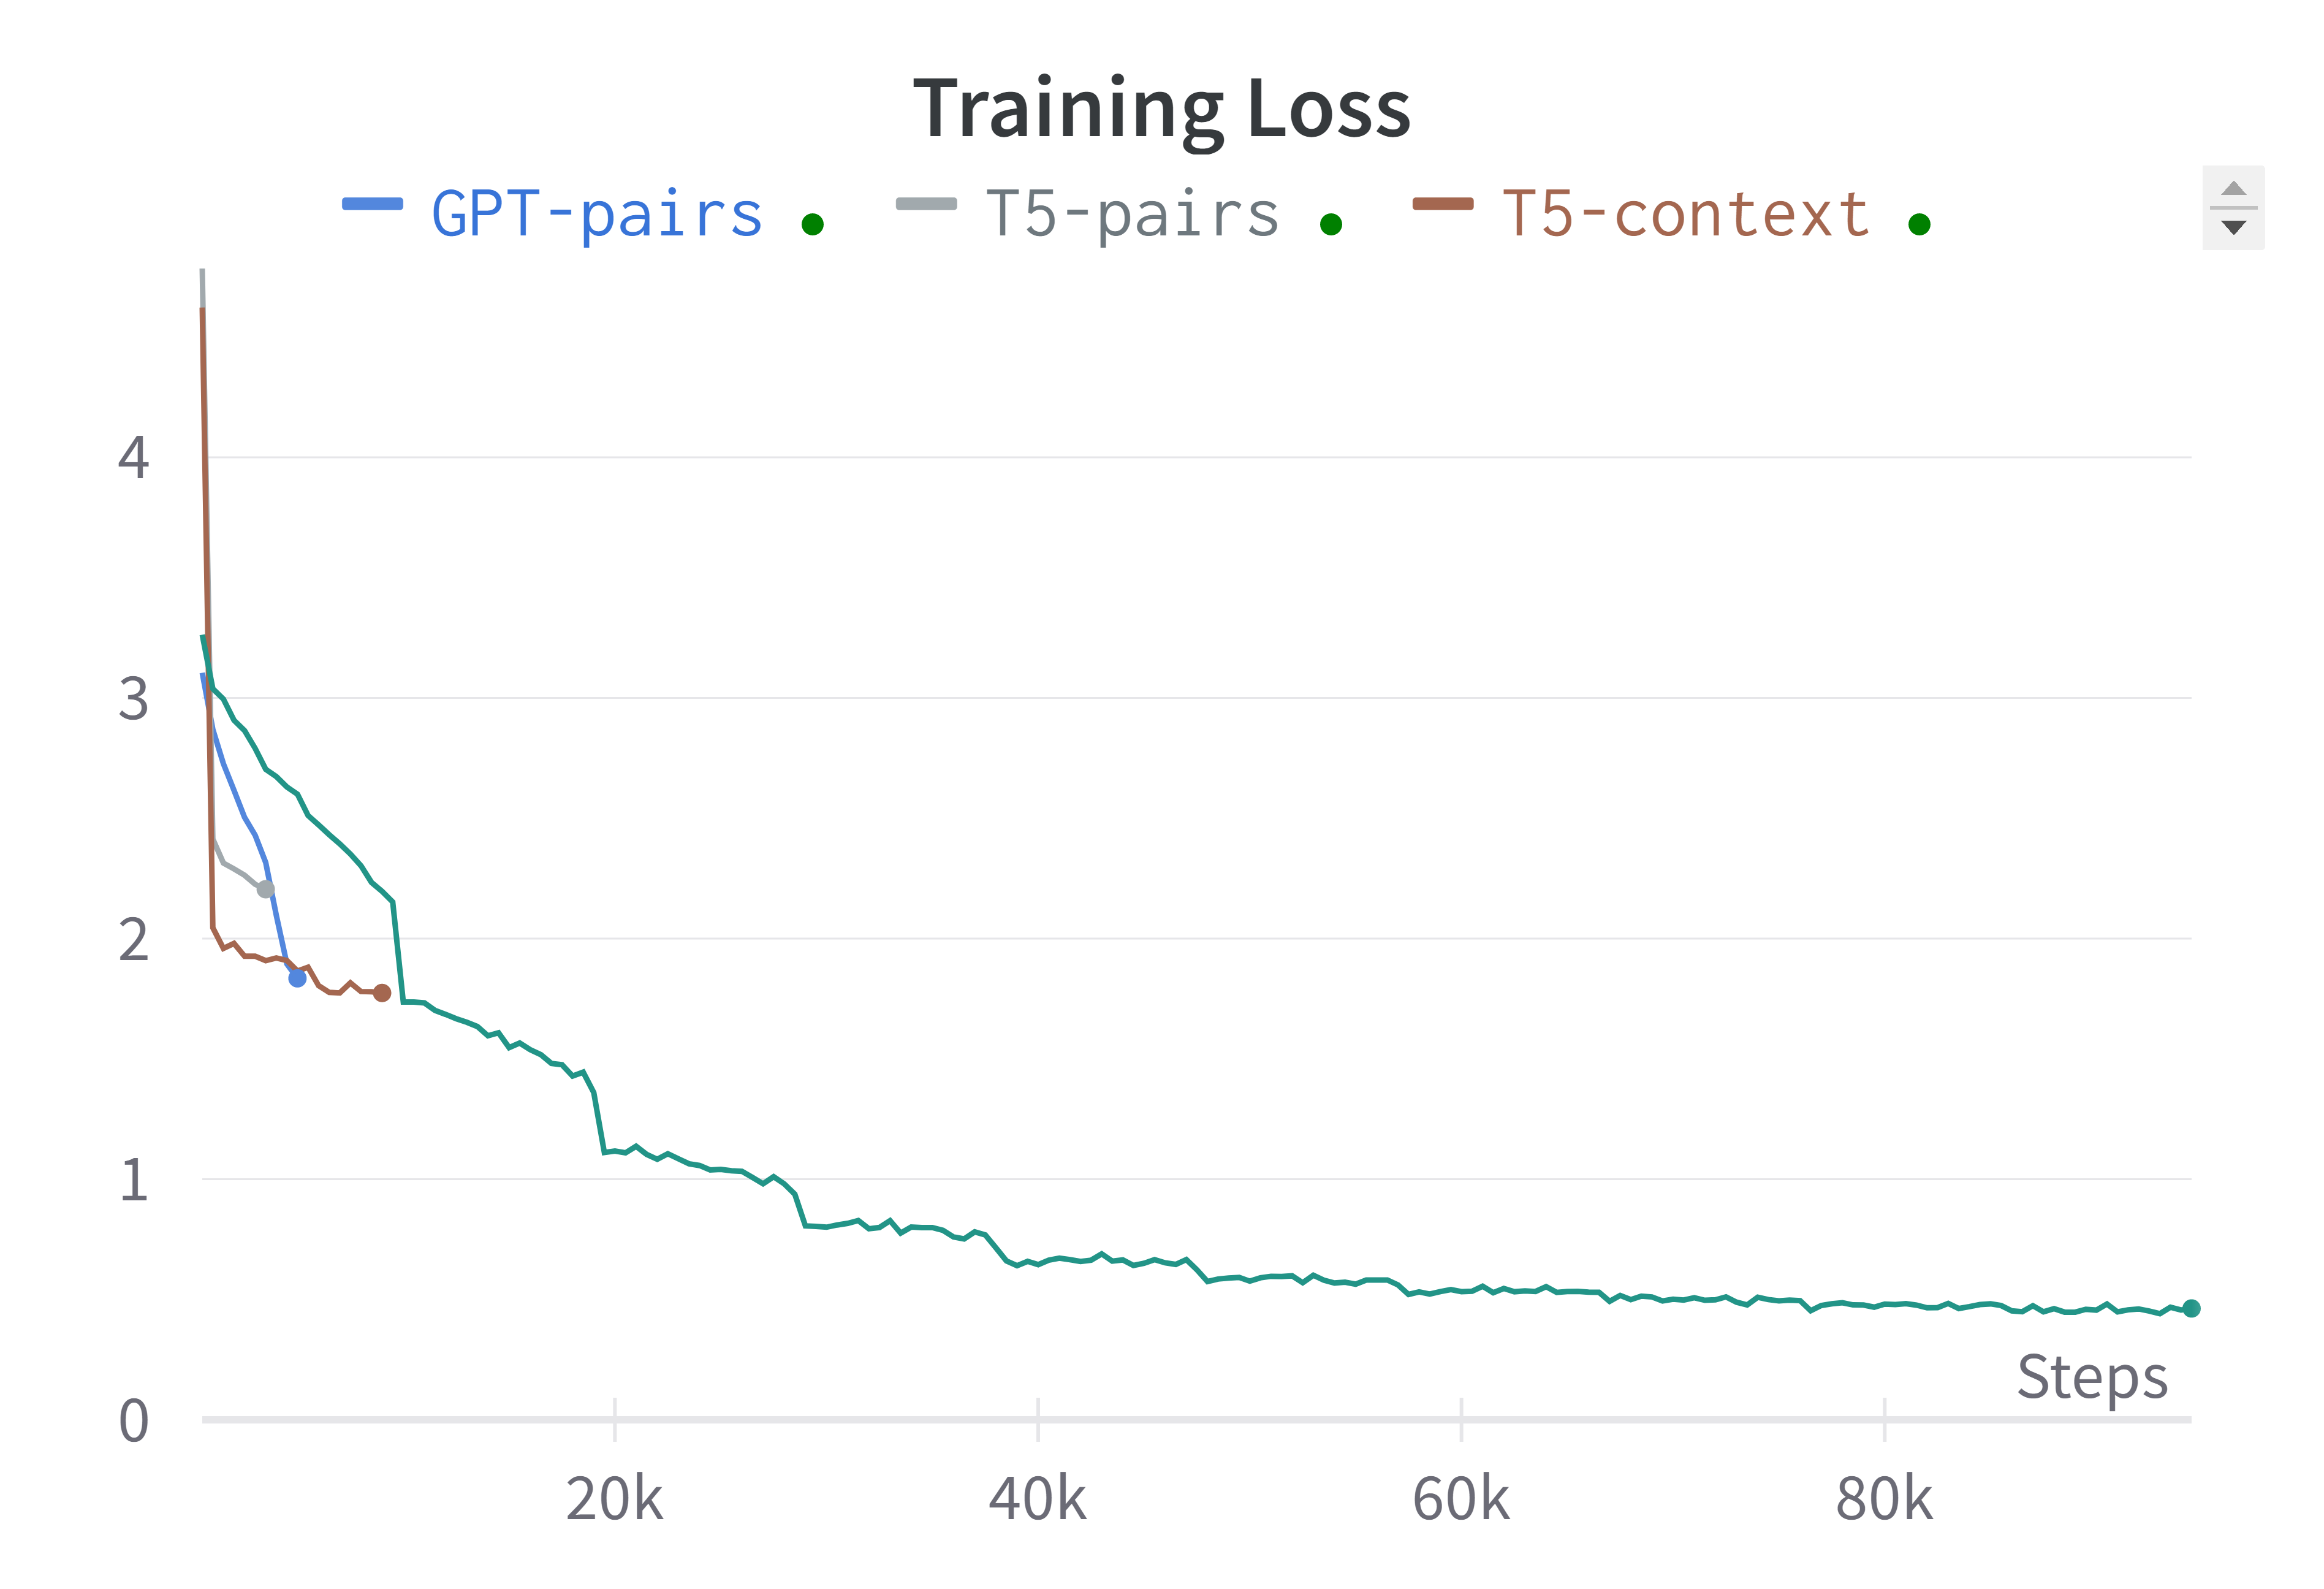
\includegraphics[width=\linewidth]{fig/training_loss.png}
	\caption{\textbf{A random visualization.} This is an example of a figure that spans only across one of the two columns.}
	\label{fig:column}
\end{figure}

% On the other hand, \figurename~\ref{fig:whole} is an example of a figure that spans across the whole page (across both columns) of the report.

% \begin{figure*} makes the figure take up the entire width of the page
% \begin{figure*}[ht]\centering 
% 	\includegraphics[width=\linewidth]{whole_page.pdf}
% 	\caption{\textbf{Visualization of a Bayesian hierarchical model.} This is an example of a figure that spans the whole width of the report.}
% 	\label{fig:whole}
% \end{figure*}


% Use the table environment to insert tables.

%\begin{table}[hbt]
%	\caption{Table of grades.}
%	\centering
%	\begin{tabular}{l l | r}
%		\toprule
%		\multicolumn{2}{c}{Name} \\
%		\cmidrule(r){1-2}
%		First name & Last Name & Grade \\
%		\midrule
%		John & Doe & $7.5$ \\
%		Jane & Doe & $10$ \\
%		Mike & Smith & $8$ \\
%		\bottomrule
%	\end{tabular}
%	\label{tab:label}
%\end{table}

% You can also insert short code examples. You can specify them manually, or insert a whole file with code. Please avoid inserting long code snippets, advisors will have access to your repositories and can take a look at your code there. If necessary, you can use this technique to insert code (or pseudo code) of short algorithms that are crucial for the understanding of the manuscript.

%\lstset{language=Python}
%\lstset{caption={Insert code directly from a file.}}
%\lstset{label={lst:code_file}}
%\lstinputlisting[language=Python]{code/example.py}

%\lstset{language=R}
%\lstset{caption={Write the code you want to insert.}}
%\lstset{label={lst:code_direct}}
%\begin{lstlisting}
%import(dplyr)
%import(ggplot)
%
%ggplot(diamonds,
%	   aes(x=carat, y=price, color=cut)) +
% geom_point() +
%  geom_smooth()
%\end{lstlisting}

%------------------------------------------------

\section*{Results}

% Use the results section to present the final results of your work. Present the results in a objective and scientific fashion. Use visualisations to convey your results in a clear and efficient manner. When comparing results between various techniques use appropriate statistical methodology.

    \textbf{TODO: describe the used metrics - currently rogue and bertscore}


    % OPTIMISTIC TABLE - all models (if they train in time)
    \begin{table*}[hbt]
    	\caption{TODO.}
    	\centering
        \scalebox{1}{
    	\begin{tabular}{c l | c c c | c c c c}
            
            &       & \multicolumn{3}{c|}{Bertscore} & \multicolumn{4}{c}{ROUGE} \\
            & Model & Precision & Recall & F1        &  rouge1 & rouge2 & rougeL & rougeLsum \\
    		\hline
            \multirow{5}{*}{\STAB{\rotatebox[origin=c]{90}{t5-small}}}
            & baseline         & & & & & & & \\
            & pairs       & & & & & & & \\
            & conv        & & & & & & & \\
            & pairs-RRHF  & & & & & & & \\
            & conv-RRHF   & & & & & & & \\
            \hline
            \multirow{5}{*}{\STAB{\rotatebox[origin=c]{90}{t5-large}}}
            & baseline         & & & & & & & \\
            & pairs       & & & & & & & \\
            & conv        & & & & & & & \\
            & pairs-RRHF  & & & & & & & \\
            & conv-RRHF   & & & & & & & \\
            \hline
            \multirow{5}{*}{\STAB{\rotatebox[origin=c]{90}{GPT2}}}
            & baseline         & & & & & & & \\
            & pairs       & & & & & & & \\
            & conv        & & & & & & & \\
            & pairs-RRHF  & & & & & & & \\
            & conv-RRHF   & & & & & & & \\
            
    	\end{tabular}
        }
    	\label{tab:results}
    \end{table*}

    % WITH LESS MODELS
    % \begin{table*}[hbt]
    % 	\caption{TODO.}
    % 	\centering
    %     \scalebox{1}{
    % 	\begin{tabular}{l | c c c | c c c c}
            
    %               & \multicolumn{3}{c|}{Bertscore} & \multicolumn{4}{c}{ROUGE} \\
    %         Model & Precision & Recall & F1        &  rouge1 & rouge2 & rougeL & rougeLsum \\
    % 		\hline
    %         t5-small         & & & & & & & \\
    %         t5-small-fine-pairs       & & & & & & & \\
    %         t5-small-fine-pairs-RRHF  & & & & & & & \\
    %         \hline
    %         GPT2         & & & & & & & \\
    %         GPT2-fine-pairs       & & & & & & & \\
    %         GPT2-fine-pairs-RRHF  & & & & & & & \\
            
    % 	\end{tabular}
    %     }
    % 	\label{tab:results}
    % \end{table*}
    


    %-------------------------
    \subsection*{Qualitative results}
    \textbf{TODO: examples of well generated sequences for prompts, example(s) of bad ones - maybe ones where we can explain why they are bad. Maybe the "Kdo je France Prešeren?" example?}

    Our plans for evaluation are comparison of responses to ChatGPT in Slovene and OpenAssistant replies translated to Slovene. We plan to do a qualitative comparison of 10 replies for each model, which will be scored by users who will not know which model produced the reply.
    Additionally we consider inspecting similarity and correlations of BERT embeddings for the model replies.

    \textbf{TODO: chery-pick the examples: THIS IS WHERE WE LOOK GOOD}

    \begin{table*}[hbt]
    	\caption{TODO.}
    	\centering
        \scalebox{1}{
    	\begin{tabular}{l}

            % PROMPT 1
            \textbf{Prompt}: Kdo je France Prešeren? \\
            \textbf{Reply}: France Prešeren je bil francoski pesnik, ki se je rodil leta 1922 v Parizu. \\
            \textbf{Reply ChatGPT}: TODO \\
            \textbf{Reply Open Assistant}: TODO \\
            \hline
            % PROMPT 2
            \textbf{Prompt}: Kdo je France Prešeren? \\
            \textbf{Reply}: France Prešeren je bil francoski pesnik, ki se je rodil leta 1922 v Parizu. Bil je francoski pisatelj in pisatelj,\\
            znan po svojem delu in delu v različnih delih sveta. \\
            \textbf{Reply ChatGPT}: TODO \\
            \textbf{Reply Open Assistant}: TODO \\
            \hline
            % PROMPT 3
            \textbf{Prompt}: Kdo je France Prešeren? \\
            \textbf{Reply}: France Prešeren je bil francoski pesnik, ki se je rodil leta 1922 v Parizu. Bil je francoski pisatelj in pisatelj,\\
            znan po svojem delu in delu na področju glasbe, glasbe in glasbe. \\
            \textbf{Reply ChatGPT}: TODO \\
            \textbf{Reply Open Assistant}: TODO \\
            
    	\end{tabular}
        }
    	\label{tab:results_qualitative}
    \end{table*}

%------------------------------------------------

\section*{Discussion}

% Use the Discussion section to objectively evaluate your work, do not just put praise on everything you did, be critical and exposes flaws and weaknesses of your solution. You can also explain what you would do differently if you would be able to start again and what upgrades could be done on the project in the future.




    %-------------------------
    \subsection*{Future work}
    % FURTHER WORK
    % Plan for enriching dataset
    For future work, combining translations from multiple sources and back-translation could improve the consistency and coherence of the conversational data.
    
    Furthermore, conducting manual inspection to identify specific linguistic nuances and subtle information that may have been lost in the translation process. This involves closely examining the messages for wordplay, understanding error messages, and capturing the underlying semantics accurately. 
    Additionally, we will explore the transformation of message formality by applying lemmatization techniques. By changing the prompts from a more formal style to an informal and conversational tone, we aim to create a dataset that better aligns with natural language interactions and user preferences.
    
    These future research directions will contribute to the refinement and enhancement of translated datasets, facilitating improved performance and user experiences in multilingual conversational applications especially for few resource languages such as Slovene.
    
    \textbf{TODO: Add more parameters!}
    LLaMA (7B)
     If we are to use the LLaMA model, we are still considering additional Slovenian pretraining on the following corpora; Gigafida~\cite{11356/1320} and ccKRES~\cite{ccKres}, we also consider the Šolar corpus \cite{kosem2011slovenian}, with considerations that the written language of primary and high school students could potentially have an impact on the models performance, and GOS \cite{Verdonik2013} with similar considerations about spoken language.


%------------------------------------------------

\section*{Conclusion}


%------------------------------------------------

% \section*{Acknowledgments}

% Here you can thank other persons (advisors, colleagues ...) that contributed to the successful completion of your project.


%----------------------------------------------------------------------------------------
%	REFERENCE LIST
%----------------------------------------------------------------------------------------
\bibliographystyle{unsrt}
\bibliography{report}


\end{document}